\documentclass[a4paper,10pt,twocolumn]{ltjsarticle}
\usepackage[haranoaji]{luatexja-preset}
\usepackage[top=18mm,bottom=20mm,left=17mm,right=17mm,columnsep=8mm]{geometry}
\usepackage{graphicx,booktabs,array,caption,enumitem,xcolor,tikz}
\usetikzlibrary{shapes.geometric}
\setlength{\parindent}{1\zw}
\renewcommand{\baselinestretch}{1.0}
\setlength{\parskip}{0pt}
\renewcommand{\thesection}{\arabic{section}.}
\renewcommand{\thesubsection}{\arabic{section}.\arabic{subsection}.}
\makeatletter
\renewcommand{\section}{\@startsection{section}{1}{\z@}{1.1\Cvs \@plus.4\Cdp \@minus.2\Cdp}{.5\Cvs \@plus.2\Cdp}{\normalfont\gtfamily\bfseries\large}}
\renewcommand{\subsection}{\@startsection{subsection}{2}{\z@}{.8\Cvs \@plus.3\Cdp \@minus.2\Cdp}{.3\Cvs \@plus.1\Cdp}{\normalfont\gtfamily\bfseries\normalsize}}
\makeatother
\captionsetup{font={small,sf},labelsep=space,justification=raggedright,singlelinecheck=false,skip=3pt}
\captionsetup[table]{position=top}
\setlist[itemize]{leftmargin=1.2\zw,itemsep=0pt,topsep=2pt,parsep=0pt}
\setlength{\textfloatsep}{8pt plus 2pt minus 2pt}
\setlength{\floatsep}{8pt plus 2pt minus 2pt}
\setlength{\intextsep}{8pt plus 2pt minus 2pt}
\pagestyle{plain}
\raggedbottom
\begin{document}
\twocolumn[{
\noindent\fbox{\gtfamily\small\ 生成AI論文\ }\par\medskip
\begin{center}
{\gtfamily\bfseries\LARGE 【TIMSS】日本の小学校4年算数・中学校2年数学の平均得点と男女差の推移（1995〜2023年）$^{\dagger}$}\par\medskip
{\gtfamily\bfseries\large 30年間の男女得点差の推移と学年・調査年による違い}\par\medskip
{\normalsize EduData調査研究グループ$^{*1}$・教育データサイエンス解析班$^{*2}$}\par
{\small オープン教育統計推進プロジェクト$^{*1}$・初等中等STEM教育データ基盤ユニット$^{*2}$}
\end{center}\smallskip
\noindent\begin{minipage}{\textwidth}\small IEAのTIMSS 2023公表値を用い，日本の小学校4年の算数と中学校2年の数学について，男女の平均得点差（男子−女子）を1995年から2023年の7時点で整理した．差は小4で0〜10点，中2で−3〜13点の範囲にあり，2023年の差（小4が10点，中2が13点）は両学年とも7時点の中で最も大きかったが，これは7時点のうち最後の1点である．2023年を除く6時点の差の平均は小4で2.3点，中2で3.5点であった．同じ30年間に男女とも平均得点は上がり，差の変化は小4で2点，中2で5点であった．使えるデータに標準誤差はなく，差が偶然の範囲かは判定できない．集計値の記述であり，要因は特定できない．\par\smallskip
\noindent{\gtfamily キーワード：}TIMSS，男女差，算数，数学，国際比較\end{minipage}\medskip
}]
\let\thefootnote\relax
\footnotetext{\footnotesize 2026年10月執筆\\ $^{\dagger}$Trends in Gender Gaps in Mathematics Scores in Japan (1995-2023) based on TIMSS Public Values†\\ $^{*1}$ Open Education Data Project, Tokyo, Japan\quad $^{*2}$ Educational Data Science Unit, Tokyo, Japan}
\section{はじめに}
\subsection{研究の背景}
算数・数学の得点の男女差は，国際的に多くの研究がある．Hyde et al. (2008)は，数学の成績で男女が似ていることを示した．Lindberg et al. (2010)は男女差の時間的な傾向を，Else-Quest et al. (2010)は国による違いを，それぞれメタ分析で調べた．Guiso et al. (2008)は文化と男女の数学の成績の関係を論じている．差の背景として，Spencer et al. (1999)はステレオタイプ脅威が女性の数学の成績に関わる可能性を論じ，Blickenstaff (2005)は理系の進路における女性の少なさを論じた．これらは差の理由を考える枠組みであり，本研究のデータで検証するものではない．

日本については，国立教育政策研究所 (2021)がTIMSS 2019の結果を報告し，Mullis et al. (2020)が同調査の国際結果を示している．本研究は，IEAが公表したTIMSS 2023の男女別平均得点を用い，日本の小4と中2について，30年間の男女差の推移を記述する．
\subsection{リサーチクエスチョン}
本研究の目的は，日本の小学校4年と中学校2年における男女の平均得点差（男子−女子）の推移を記述し，学年と調査年による違いを整理することである．
\begin{itemize}
\item RQ1：日本の小学校4年と中学校2年で，男子と女子の平均得点の差（男子−女子）は1995年から2023年にかけてどう推移したか．
\item RQ2：男女得点差は，学年と調査年によってどのように異なるか（標本調査の誤差を踏まえて）．
\end{itemize}
\section{調査対象および分析方法}
IEAのTIMSS 2023 International Results in Mathematics and Scienceの公表値を用いた．対象は日本の小学校4年の算数と中学校2年の数学で，調査年は各学年7時点（1995，2003，2007，2011，2015，2019，2023年），計14観測である．中2の1999年は男女別の公表がないため含めない．各調査は学校を抽出し学級単位で行う標本調査で，各回の対象は各学年約4000〜5000人である．得点は整数で公表されている．

男女得点差は「男子平均−女子平均」とし，学年ごとに時点を同じ重みで扱った．公表値は整数のため，差には±1点程度の丸めの影響がありうる．本研究が使ったデータに標準誤差は含まれておらず，有意性の検定は行わない．調査年の間隔は，1995年から2003年が8年，その後は4年であり，時点を同じ重みで扱った平均は，間隔の違いを考慮していない．男女得点差は男子と女子の平均から計算した値なので，これらの間の相関は結果にしない．相関の探索も行っていないため，多重比較の補正は要しない．特定の時点への依存は，2023年を除いた平均と，1時点ずつ除いた平均で確かめた．
\begin{table*}[!t]
\caption{主要指標の基本記述統計量}
\centering\small
\begin{tabular}{>{\raggedright\arraybackslash}p{9.2cm}rrrrrr}
\toprule
指標 & \textit{K} & 平均 & \textit{SD} & 中央値 & 最小 & 最大 \\
\midrule
平均得点 & 2 & 593.0 & 2.8 & 593.0 & 591.0 & 595.0 \\
男子平均得点 & 2 & 598.5 & 3.5 & 598.5 & 596.0 & 601.0 \\
女子平均得点 & 2 & 587.0 & 1.4 & 587.0 & 586.0 & 588.0 \\
男女得点差 & 2 & 11.5 & 2.1 & 11.5 & 10.0 & 13.0 \\
\bottomrule
\end{tabular}
\par\smallskip{\footnotesize 注）単位は点，\textit{K}は観測数（国・地域・区分）．2023年度の断面．}
\end{table*}
\begin{table*}[!t]
\caption{主要指標間のピアソンの相関係数と，ベイズファクター}
\centering\small
\begin{tabular}{>{\raggedright\arraybackslash}p{6.4cm}>{\raggedright\arraybackslash}p{6.4cm}rrr}
\toprule
指標 \textit{X} & 指標 \textit{Y} & \textit{r} & \textit{p} & \textit{BF}\textsubscript{10} \\
\midrule

\bottomrule
\end{tabular}
\par\smallskip{\footnotesize 注）\textit{BF}\textsubscript{10}はJZSベイズファクター（3を超えれば関連を支持，1/3を下回れば関連がないことを支持）．全ペアの探索の一部を載せた．}
\end{table*}
\section{結果}
RQ1．小4の差は，1995年から順に8，3，0，3，0，0，10点であった．中2の差は，同じ順に8，2，4，8，−3，2，13点であった．14観測のうち，差が正は10，0は3（小4の2007，2015，2019年），負は1（中2の2015年，女子588点，男子585点）であった．1995年から2023年への差の変化は，小4で+2点，中2で+5点であった．2023年の差は両学年とも7時点で最大で，次に大きい値はどちらも1995年の8点であった．2023年を除く6時点の差の平均は，小4で2.3点，中2で3.5点である．

男女の平均得点は，1995年から2023年に小4で男子が571点から596点（+25），女子が563点から586点（+23），中2で男子が585点から601点（+16），女子が577点から588点（+11）に上がった．男女計の平均は小4で567点から591点（+24），中2で581点から595点（+14）である．差の変化（+2点，+5点）は，平均得点の変化より小さい．ただし2019年から2023年にかけては，女子が小4で7点，中2で5点下がり，男子は小4で3点，中2で6点上がっており，これが2023年の差を広げた．

RQ2．同じ年で比べると，中2の差が小4より大きいのは4時点（2007，2011，2019，2023年），小4が大きいのは2時点（2003，2015年），等しいのは1995年である．7時点の平均は小4で3.4点，中2で4.9点であった．差が3点以下の時点は，小4で5，中2で3ある．この大きさの差は，丸めや抽出のばらつきと区別できない．標準誤差がないため，ほかの時点も偶然の範囲かどうかは判定できない．

特定の時点への依存を調べた．1時点ずつ除いた7時点の平均差は，小4で2.3〜4.0点，中2で3.5〜6.2点で，どれも正であった．規模が小さい区分や注意が付いた項目は，このデータにはない．
\begin{figure}[t]\centering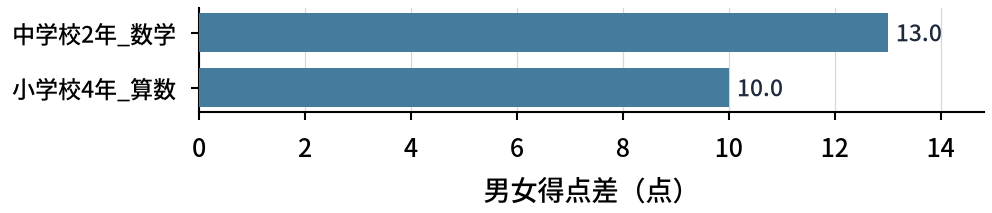
\includegraphics[width=\columnwidth]{chart_japan_timss_math_science.png}\caption{男女得点差の値の比較．赤が日本}\end{figure}
\begin{figure}[t]\centering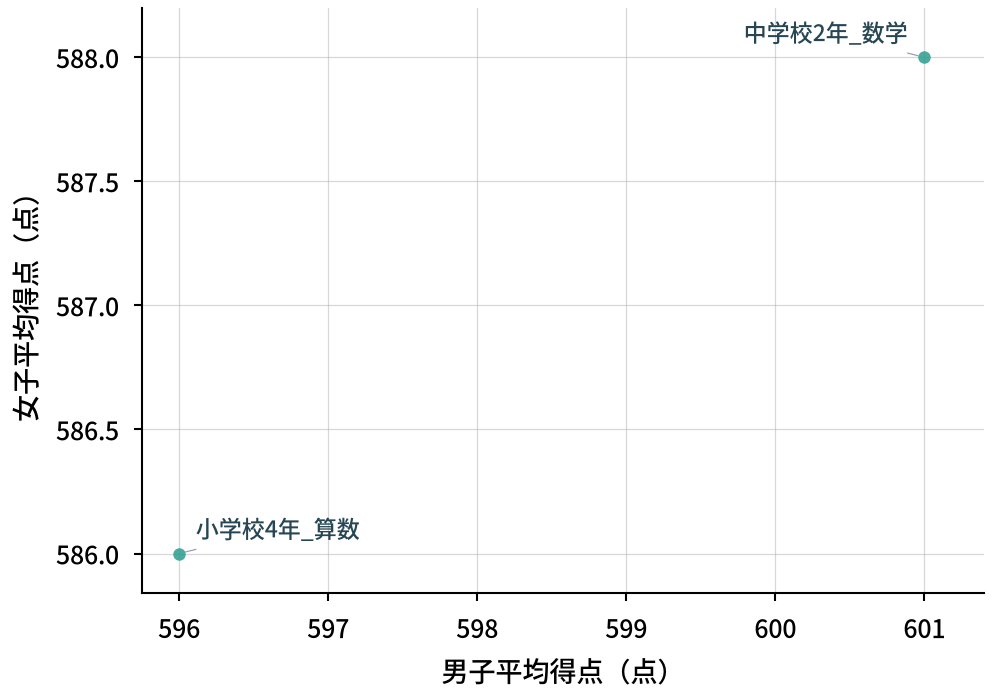
\includegraphics[width=\columnwidth]{chart_secondary_japan_timss_math_science.png}\caption{男子平均得点と女子平均得点の関連（回帰直線と，その平均の95\%信頼区間の帯，n=2）}\end{figure}
\section{考察}
男女の平均得点差は，30年間で0点前後から十数点の幅で動き，2023年は両学年で最大であった．Hyde et al. (2008)が示した男女の類似性と並べると，差が3点以下の時点が多いことは，それと矛盾するとは言えない．ただし，本研究は点差を得点のばらつきで割った効果量を持たないため，Hyde et al. (2008)と同じ尺度で比べたものではない．一方，Lindberg et al. (2010)のように時間的な傾向を見る立場からは，2023年の拡大は注意して見るべき点である．ただし，この拡大は7時点のうちの最後の1点であり，標準誤差もないため，傾向の始まりか，ばらつきの範囲かは本研究では分からない．拡大は，女子の平均が2019年より下がり，男子が上がったことで生じていた．

差の背景として，Spencer et al. (1999)が論じたステレオタイプ脅威や，Guiso et al. (2008)が論じた文化の違い，学習環境などが考えられる．しかし本研究は男女別の平均得点しか使っておらず，これらは仮説にとどまる．Else-Quest et al. (2010)が国による違いを示したように，差は社会の文脈で変わりうるが，日本一国の7時点では検証できない．Blickenstaff (2005)が扱う進路との関係も，本データでは調べていない．2023年の差の拡大を読むには，国立教育政策研究所 (2021)やMullis et al. (2020)が扱うTIMSS 2019の報告と合わせ，標準誤差つきの公式の表で確かめる必要がある．

限界は，(1)学年と性別ごとの平均の集計値のみで，個々の生徒の関連は示せないこと，(2)標本調査で標準誤差がなく，丸めの影響もあること，(3)指導内容や社会的要因などの交絡を統制していないこと，(4)時点が各学年7で，傾向の検定ができないこと，(5)中2の1999年がないこと，である．教育現場への示唆として，男女差に応じた指導の効果は，本研究では確かめられていない．
\section*{参考文献}
\begingroup\scriptsize\raggedright\interlinepenalty=10000 
\begin{list}{}{\setlength{\leftmargin}{1.5\zw}\setlength{\itemindent}{-1.5\zw}\setlength{\labelwidth}{0pt}\setlength{\labelsep}{0pt}\setlength{\itemsep}{1pt}\setlength{\parsep}{0pt}\setlength{\topsep}{0pt}\setlength{\listparindent}{0pt}}
\item BLICKENSTAFF, J. C. (2005) Women and science careers: Leaky pipeline or gender filter? Gender and Education, \textbf{17} (4) ：369-386.
\item ELSE-QUEST, N. M., HYDE, J. S. and LINN, M. C. (2010) Cross-national patterns of gender differences in mathematics: A meta-analysis. Psychological Bulletin, \textbf{136} (1) ：103-127.
\item GUISO, L., MONTE, F., SAPIENZA, P. and ZINGALES, L. (2008) Culture, gender, and math. Science, \textbf{320} (5880) ：1164-1165.
\item HYDE, J. S., LINDBERG, S. M., LINN, M. C., ELLIS, A. B. and WILLIAMS, C. C. (2008) Gender similarities characterize math performance. Science, \textbf{321} (5888) ：494-495.
\item 国立教育政策研究所 (2021) 算数・数学教育／理科教育の国際比較：TIMSS 2019 国際数学・理科教育動向調査の2019年調査報告書. 明石書店.
\item LINDBERG, S. M., HYDE, J. S., PETERSEN, J. L. and LINN, M. C. (2010) New trends in gender and mathematics performance: A meta-analysis. Psychological Bulletin, \textbf{136} (6) ：1123-1135.
\item MULLIS, I. V. S., MARTIN, M. O., FOY, P., KELLY, D. L. and FISHBEIN, B. (2020) TIMSS 2019 International Results in Mathematics and Science. Boston College, TIMSS \& PIRLS International Study Center.
\item SPENCER, S. J., STEELE, C. M. and QUINN, D. M. (1999) Stereotype threat and women's math performance. Journal of Experimental Social Psychology, \textbf{35} (1) ：4-28.
\end{list}\endgroup
\section*{Summary}
{\footnotesize\setlength{\parindent}{0pt}Using TIMSS 2023 published values, this study describes the gender gap (male minus female) in mean mathematics scores of Japanese 4th-grade and 8th-grade students at seven time points from 1995 to 2023. The gap ranged from 0 to 10 points in grade 4 and from −3 to 13 points in grade 8, and the 2023 gap was the largest of the seven in both grades. Standard errors were not available, so whether the gaps exceed sampling variation could not be judged. The study is descriptive and does not attribute causes.\par\smallskip KEYWORDS: TIMSS, Gender Gap, Mathematics, Japan, International Comparison\par}
\medskip\noindent\fbox{\parbox{\dimexpr\columnwidth-2\fboxsep-2\fboxrule}{\footnotesize\gtfamily 【付記：生成AIによる自動執筆に関する開示】\\ 本論文は学生への教育目的で作成している．使用しているデータは公的オープンデータである．統計の算出はPythonで行い，文章は生成AI（Anthropic Claude等）を活用して作成した．記載した統計数値は元データに準拠しているが，教育学的な考察や提言の妥当性は，指導現場の実情に応じて，批判的に吟味してほしい．}}
\end{document}
